\section{Results}
\label{sec:results}

We tested our methods on twenty different $512\times 512$ gray scale images, each with nine different masks of missing pixels. Each mask consisted randomly missing pixels from 10\% to 90\%.

We compare algorithms based on two criteria: the mean-squared error of the original image compared to the reconstructed image and the runtime of the algorithm. The following six inpainting algorithms have been tested:
\begin{enumerate}
	\item Sparse-coding with a DCT dictionary.
	\item Sparse-coding with a learned dictionary.
	\item Singular Value Decomposition.
	\item Regular diffusion with a $K_{\text{diamond}}$ kernel.
	\item Regular diffusion with a $K_{\text{gauss}}$ kernel.
	\item Directional diffusion with patches of size $32 \times 32$.
\end{enumerate}

\begin{figure*}
	\begin{subfigure}[b]{0.48\textwidth}
		\centering
		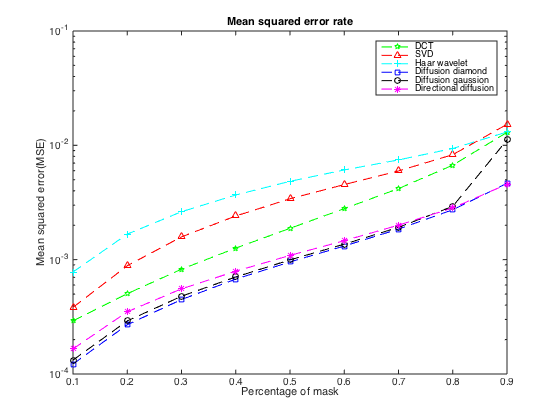
\includegraphics[trim=1.4cm 0.5cm 1.5cm 0.5cm, clip, width=0.9\textwidth]{figures/mse}
		\caption{Mean square error }
		\label{fig:mse}
	\end{subfigure}
	\begin{subfigure}[b]{0.48\textwidth}
		\centering
		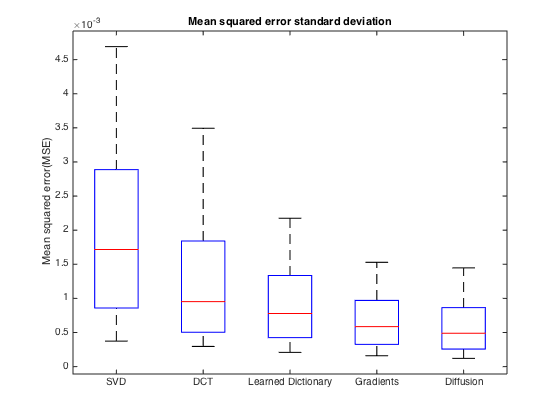
\includegraphics[trim=1.4cm 0.5cm 1.5cm 0.5cm, clip, width=0.9\textwidth]{figures/mse_std}
		\caption{Standard deviation of mean squared error}
		\label{fig:mse_std}	
	\end{subfigure}
\end{figure*}


\begin{figure}
		
\end{figure}